\documentclass[hyperref={colorlinks}]{beamer}

\usepackage{graphicx}
\usepackage{amsfonts,amsmath,color}       
\usepackage[spanish,activeacute]{babel}
\usepackage[utf8]{inputenc}
\usepackage{tikz}
\usetikzlibrary{mindmap,trees}
\usetikzlibrary{decorations.text,calc,arrows.meta}
\usepackage{colortbl}
\usepackage{listings}
\lstset{basicstyle=\footnotesize\ttfamily,escapeinside={\%*}{*)}}
\usepackage{fancyvrb}

\usefonttheme{professionalfonts}
\usetheme{Warsaw}

%\setbeamertemplate{caption}[numbered]
%\setbeamercovered{dynamic}

%\beamertemplatenavigationsymbolsempty

\begin{document}
\title{Introducci\'on a GNU/Linux}
\author{Guillermo Rubilar}
\institute{\tiny [Confeccionado usando parte del c\'odigo fuente disponible en \url{https://github.com/giomba/beamer-intro-linux} y \\ \url{https://github.com/alexpacheco/linux}]}
\date{\today}




\maketitle

\begin{frame}
 \tableofcontents
\end{frame}

\section{Componentes de GNU/Linux}
\begin{frame}[fragile]
  \frametitle{Componentes de GNU/Linux}
  \begin{columns}[T]
    \column{0.55\textwidth}
%    \begin{itemize}
%    \item Linux is made up of two (three) parts:
      \begin{itemize}
      \only<1,2>{\item Kernel} 
      \only<1,3>{\item Shell}
      \only<1,4>{\item Aplicaciones/Programas} 
      \only<2>{
        \begin{itemize}
        \item El kernel es el ``n\'ucleo"\, del sistema operativo.
        \item Es el puente entre las aplicaciones y el procesamiento de datos realizado directamente en el hardware del sistema.
        \item Una de las tareas principales del kernel es administrar los recursos del sistema.
        \end{itemize}
      }
      \only<3>{
        \begin{itemize}
        \item La ``shell'' es la interface de l\'inea de comandos, siendo la interfaz primaria  de los sistemas operativos Linux/Unix.
        \item La shell es simplemente una aplicaci\'on que corre sobre el kernel y suministra una interfaz poderosa.
        \end{itemize}
      }
      \only<4>{
        \begin{itemize}
        \item Linux suministra un gran n\'umero de aplicaciones \'utiles en el \'ambito cient\'ifico (y tambi\'en para tareas cotidianas y recreativas).
        \item La mayor\'ia de los programas disponibles para Windows tienen su equivalente o similar en Linux.
        \end{itemize}
      }
      \end{itemize}
%    \end{itemize}
    \column{0.45\textwidth}
    \begin{tikzpicture}[scale=0.75]
      \coordinate (O) at (0,0);
      \draw[fill=blue!10,blue!10] (O) circle (3.4);
      \onslide<4>{\draw[fill=blue,blue] (O) circle (3.4);}
      \draw[fill=blue!20,blue!20] (O) circle (2.6);
      \onslide<3>{\draw[fill=blue,blue] (O) circle (2.6);}
      \draw[fill=blue!30,blue!30] (O) circle (1.8);
      \onslide<2>{\draw[fill=blue,blue] (O) circle (1.8);}
      \draw[fill=blue!40,blue!40] (O) circle (1.1);

      \draw[decoration={text along path,reverse path,text align={align=center},text={Otros programas}},decorate] (2.9,0) arc (0:180:2.9);
      \draw[decoration={text along path,reverse path,text align={align=center},text={Shell}},decorate] (2.1,0) arc (0:180:2.1);
      \draw[decoration={text along path,reverse path,text align={align=center},text={Kernel}},decorate] (1.3,0) arc (0:180:1.3);
      \draw[decoration={text along path,reverse path,text align={align=center},text={Hardware}},decorate] (0.65,0) arc (0:180:0.6);
    \end{tikzpicture}
  \end{columns}
  \begin{center}
    
\includegraphics[width=.10\textwidth]{figs/gnu.pdf}
    
\includegraphics[width=.10\textwidth]{figs/tux.pdf}\\
GNU/Linux
\end{center}
\end{frame}

\section{Un poco de historia}
\begin{frame}
    \frametitle{Software libre y GNU}

    \begin{minipage}{.4\linewidth}
    \begin{figure}
    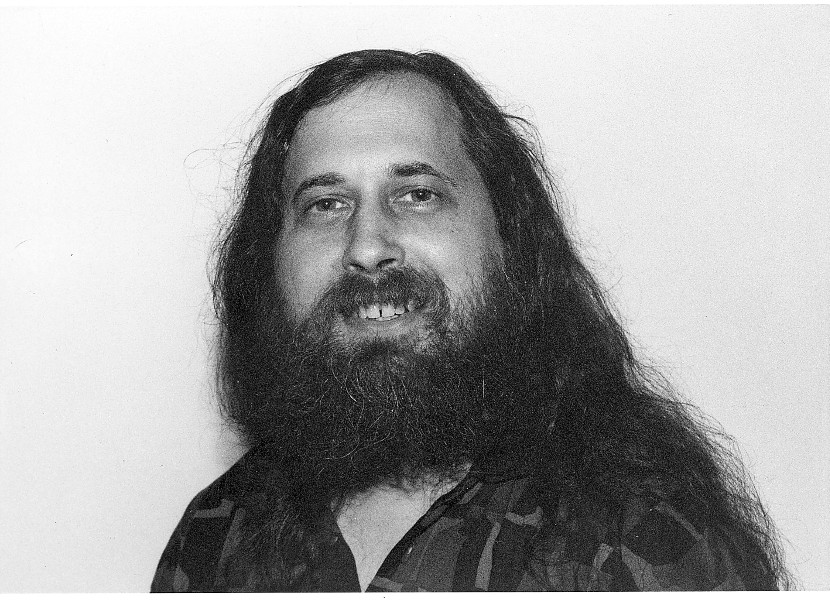
\includegraphics[width=.9\linewidth]{figs/rms.jpeg}
    \caption{Richard Stallman}
    \end{figure}
    \end{minipage}
    \pause
    \begin{minipage}{.55\linewidth}
    \begin{block}{Software libre}
        \begin{enumerate}
        \setcounter{enumi}{-1}
        \item libertad de usar el programa para cualquier prop\'osito
        \item libertad de estudiar el funcionamiento del programa
        \item libertad de poder modificar el programa
        \item libertad de poder distribuir el programa modificado
        \end{enumerate}
    \end{block}
    \pause
    \begin{block}{1984}
        \begin{minipage}{.2\linewidth}
        \visible<3->{
\includegraphics[width=1\linewidth]{figs/gnu.pdf}}
        \end{minipage}
        \begin{minipage}{.75\linewidth}
        Nace GNU, sistema operativo completamente libre, basado en Unix
        \end{minipage}
    \end{block}
    \end{minipage}
\end{frame}

\begin{frame}
    \frametitle{Linus Torvalds y Linux}

    \begin{minipage}{.4\linewidth}
    \begin{figure}
        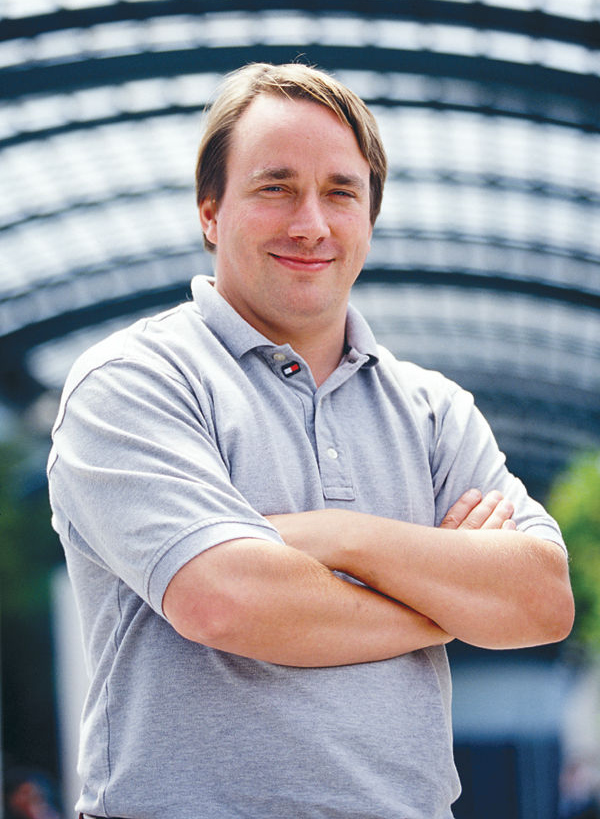
\includegraphics[width=.9\linewidth]{figs/torvalds.jpeg}
        \caption{Linus Torvalds}
        \end{figure}
    \end{minipage}
    \begin{minipage}{.55\linewidth}
        \begin{block}{El problema}
            \begin{itemize}
                \item
                    \begin{minipage}{.2\linewidth} \visible<1->{
\includegraphics[width=.9\linewidth]{figs/i-3-unix.pdf}} \end{minipage}
                    \begin{minipage}{.75\linewidth} En la universidad, es un apasionado de los sistemas Unix \end{minipage}
                    \pause
                \item
                    \begin{minipage}{.2\linewidth} \visible<2->{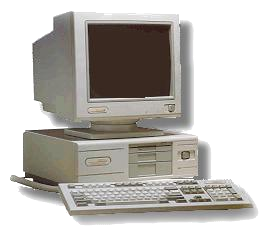
\includegraphics[width=.9\linewidth]{figs/pc-i386.png}} \end{minipage}
                    \begin{minipage}{.75\linewidth} Compra un PC i386 \end{minipage}
                    \pause
                \item
                    \begin{minipage}{.2\linewidth} \visible<3->{
\includegraphics[width=.9\linewidth]{figs/minix.pdf}} \end{minipage}
                    \begin{minipage}{.75\linewidth} Instala Minix-Unix en su PC \end{minipage}
                    \pause
                \item
                    \begin{minipage}{.2\linewidth} \visible<4->{
\includegraphics[width=.9\linewidth]{figs/error.pdf}} \end{minipage}
                    \begin{minipage}{.75\linewidth} Imposibilidad de modificar libremente Minix \end{minipage}
                    \pause
            \end{itemize}
        \end{block}
    \begin{block}{1991}
        \begin{minipage}{.2\linewidth}
        \visible<5->{
\includegraphics[width=1\linewidth]{figs/tux.pdf}}
        \end{minipage}
        \begin{minipage}{.75\linewidth}
        Nace el kernel Linux
        \end{minipage}
    \end{block}
    \end{minipage}
\end{frame}

\begin{frame}
\frametitle{El desarrollo de GNU / Linux}
\begin{center}
    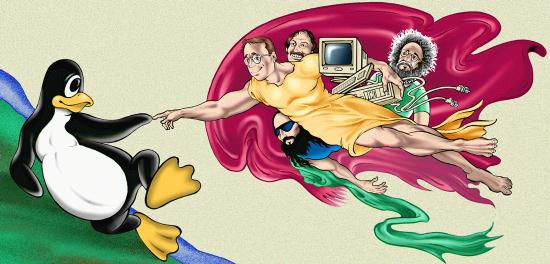
\includegraphics[width=.50\textwidth]{figs/tux21.png}\\
GNU/Linux
\end{center}
\begin{itemize}
\item 1984 -- Nace el sistema operativo GNU
\item 1991 -- Nace el kernel Linux
\item 1992 -- El kernel de Linux se libera bajo la licencia GPL
\item 1993 -- Nacen Slackware y Debian
\item 1994 -- Nacen Suse y RedHat
\item 2004 -- Nace Ubuntu
\item 2006 -- Nace Linux Mint
\end{itemize}
\end{frame}

\section{Linux hoy}
\begin{frame}
    \frametitle{Las razones del \'exito}
\begin{center}
    
\includegraphics[width=.10\textwidth]{figs/gnu.pdf}
    
\includegraphics[width=.10\textwidth]{figs/tux.pdf}\\
GNU/Linux
\end{center}

    \begin{itemize}
        \item
            \begin{minipage}{.10\linewidth} \visible<1->{
\includegraphics[width=.9\linewidth]{figs/no-cost.pdf}} \end{minipage} Gratuito \pause
        \item
            \begin{minipage}{.10\linewidth} \visible<2->{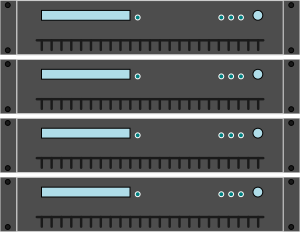
\includegraphics[width=.9\linewidth]{figs/servers.png}} \end{minipage} Soporte multiprocesadores y  multiplataforma \pause
        \item
            \begin{minipage}{.10\linewidth} \visible<3->{
\includegraphics[width=.9\linewidth]{figs/apache.png}} \end{minipage} Servidores Web (Apache) \pause
        \item
            \begin{minipage}{.10\linewidth} \visible<4->{
\includegraphics[width=.9\linewidth]{figs/redhat.png}} \end{minipage} Productos comerciales con hardware certificado 
    \end{itemize}
\end{frame}

\begin{frame}
    \frametitle{Flexibilidad}
\begin{center}
    
\includegraphics[width=.10\textwidth]{figs/tux30.png}
\includegraphics[width=.10\textwidth]{figs/tux31.png}
\includegraphics[width=.10\textwidth]{figs/tux33.png}
\end{center}

    \begin{columns}
    \begin{column}{.25\textwidth}
        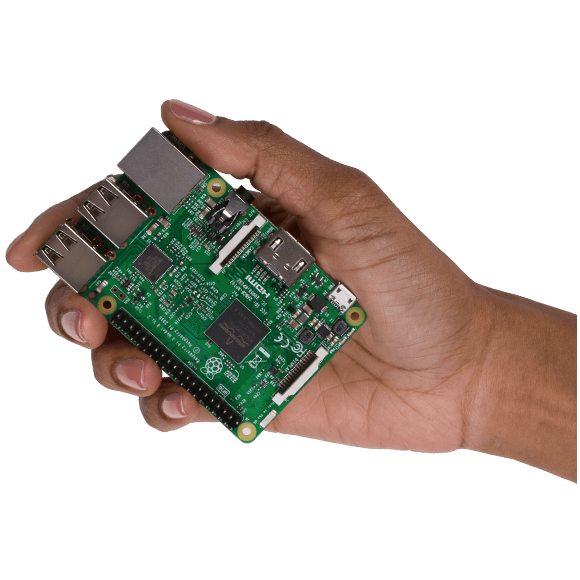
\includegraphics[width=.9\linewidth]{figs/raspberry.png}

        \centering Minicomputadoras
    \end{column}

    \begin{column}{.25\textwidth}
        
\includegraphics[width=.9\linewidth]{figs/android.png}

        \centering Tel\'efonos inteligentes
    \end{column}

    \begin{column}{.25\textwidth}
        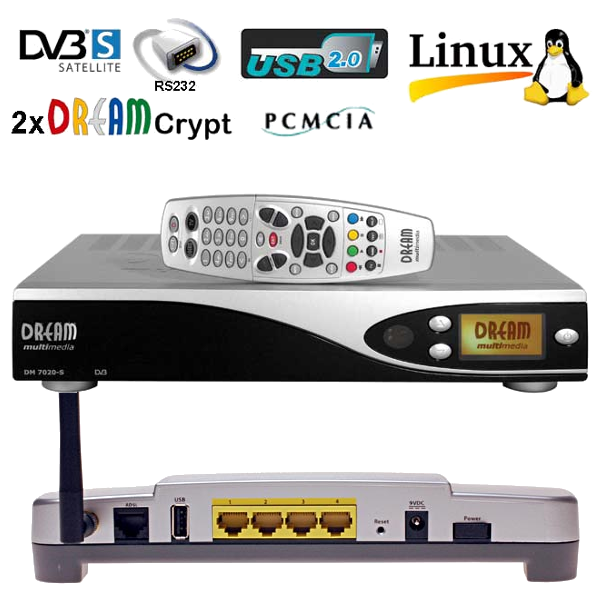
\includegraphics[width=.9\linewidth]{figs/router-decoder.png}

        \centering Modem, Router
    \end{column}
    \end{columns}

\end{frame}



\begin{frame}
    \frametitle{Distribuciones}
    \begin{itemize}
    \item Una \textbf{distribuci\'on} es un conjunto particular de software que permite instalar, configurar y utilizar el kernel linux, los programas GNU, y software adicional.
    \end{itemize}
	\begin{minipage}[b][.30\textheight][t]{.3\textwidth}
	    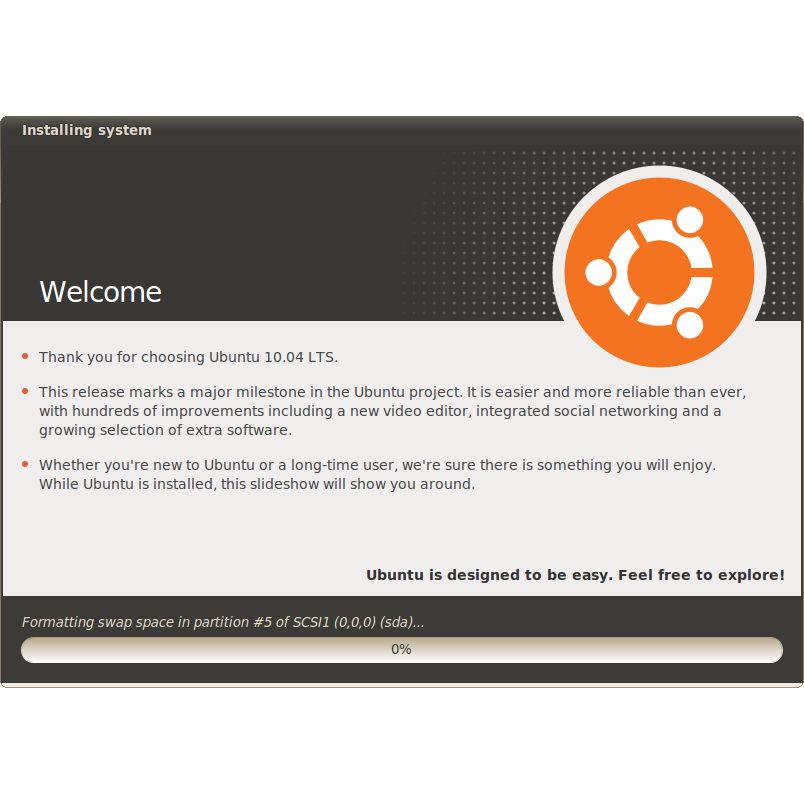
\includegraphics[width=.7\textwidth]{figs/ubiquity.png}\\
	    \centering Instalador
    \end{minipage}\hfill
    \begin{minipage}[b][.30\textheight][t]{.3\textwidth}
	    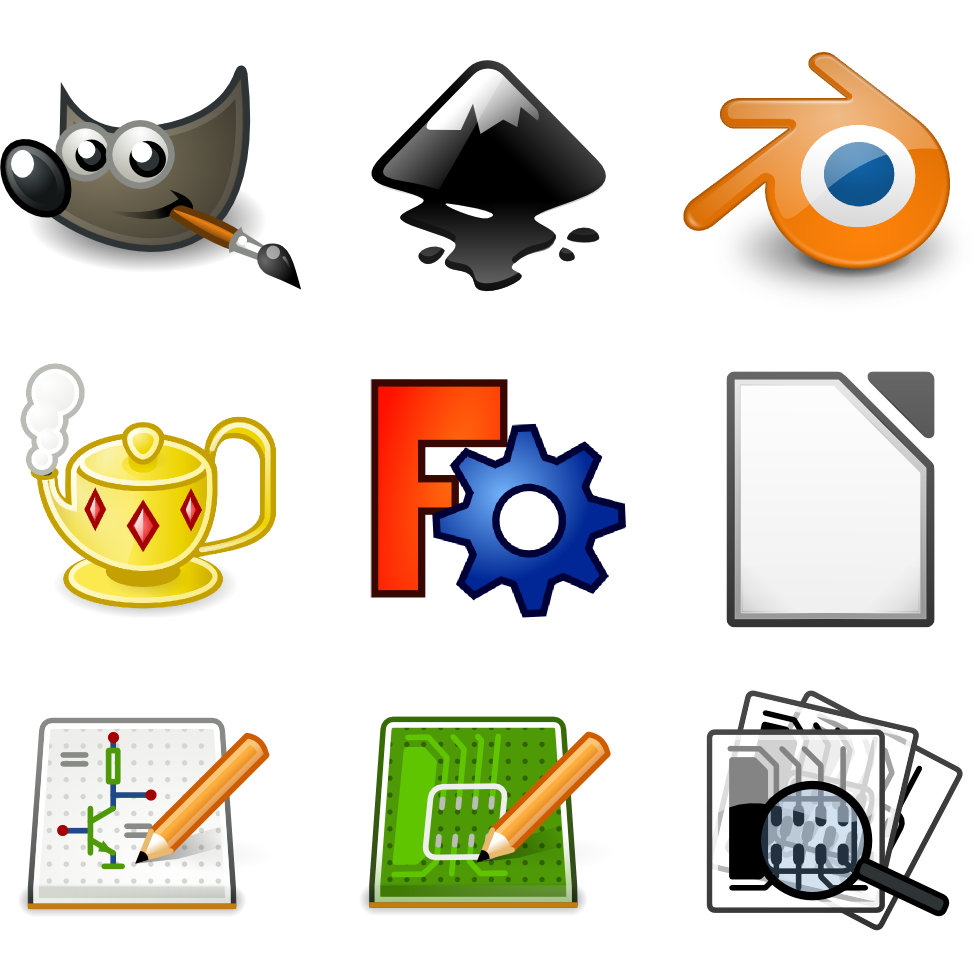
\includegraphics[width=.7\textwidth]{figs/oss.png}\\
	    \centering Utilidades 
    \end{minipage}\\
    \vspace{.10\textheight}
    \begin{minipage}[b][.30\textheight][t]{.3\textwidth}
	    
\includegraphics[width=.7\textwidth]{figs/firefox.pdf}\\
	    \centering Navegador
    \end{minipage}\hfill
    \begin{minipage}[b][.30\textheight][t]{.3\textwidth}
	    
\includegraphics[width=.7\textwidth]{figs/libreoffice.png}\\
	    \centering Programas de Oficina
    \end{minipage}
%    \begin{minipage}[b][.30\textheight][t]{.3\textwidth}
%    \includegraphics[width=.7\textwidth]{figs/mint-dvd.png}\\
%    \centering Distribuci\'on
%    \end{minipage}


\end{frame}

\begin{frame}
    \frametitle{Las distribuciones m\'as famosas}
    \begin{itemize}
    \item Existen \textit{miles de distribuciones distintas} (ver \url{www.distrowatch.com}), que difieren en la selecci\'on de programas que incluyen y su configuraci\'on.
    \end{itemize}

    \begin{minipage}[b][.30\textheight][t]{.3\textwidth}
    
\includegraphics[width=.7\textwidth]{figs/logo-debian.pdf}\\
    \end{minipage}\hfill
    \begin{minipage}[b][.30\textheight][t]{.3\textwidth}
    
\includegraphics[width=.7\textwidth]{figs/logo-ubuntu.png}\\
    \centering
    Ubuntu
    \end{minipage}\hfill
    \begin{minipage}[b][.30\textheight][t]{.3\textwidth}
    
\includegraphics[width=.7\textwidth]{figs/logo-linuxmint.pdf}\\
    \centering
    LinuxMint
    \end{minipage}\\[0.5em]

    \begin{minipage}[b][.30\textheight][t]{.3\textwidth}
    
\includegraphics[width=.7\textwidth]{figs/logo-fedora.pdf}\\
    \centering
    Fedora
    \end{minipage}\hfill
    \begin{minipage}[b][.30\textheight][t]{.3\textwidth}
    
\includegraphics[width=.7\textwidth]{figs/logo-centos.pdf}\\
    \end{minipage}\hfill
    \begin{minipage}[b][.30\textheight][t]{.3\textwidth}
    
\includegraphics[width=.7\textwidth]{figs/redhat.png}\\
    
    \end{minipage}
\end{frame}

\begin{frame}\frametitle{Entornos Gr\'aficos}
	\begin{block}{}
		\begin{itemize}
			\item KDE (\href{https://www.kde.org}{www.kde.org})
			\item GNOME (\href{https://www.gnome.org}{www.gnome.org})
			\item MATE (\href{https://www.mate-desktop.org}{www.mate-desktop.org})
			\item CINNAMON (\href{http://cinnamon.linuxmint.com}{cinnamon.linuxmint.com})
			\item XFCE (\href{https://www.xfce.org}{www.xfce.org})
			\item FLUXBOX (\href{http://fluxbox.org/}{fluxbox.org})
			\item DEEPIN (\href{https://www.deepin.org/en/dde/}{www.deepin.org/en/dde})
			\item AWESOME (\href{https://awesomewm.org/}{awesomewm.org})
			\item Etc, etc, etc. 
		\end{itemize}
	\end{block}
	\begin{block}{}
		En general, cada entorno gr'afico cuenta con sus propios programas para gestionar archivos, configurar el entorno, etc.
	\end{block}
\end{frame}


\begin{frame}
  \frametitle{Archivos y Procesos}
  \begin{itemize}
    \item En Linux/Unix \textit{todo} es un archivo o bien un proceso.
    \item Un archivo es una conjunto de datos, creados por un usuario usando alg\'un programa.
    \item Un proceso en un programa que se est'a ejecutando. Tiene asociado un c\'odigo identificador \'unico (PID).
  \end{itemize}
\end{frame}

 \tikzset{
    invisible/.style={opacity=0},
    visible on/.style={alt={#1{}{invisible}}},
    alt/.code args={<#1>#2#3}{%
      \alt<#1>{\pgfkeysalso{#2}}{\pgfkeysalso{#3}} % \pgfkeysalso doesn't change the path
    },
  }

\begin{frame}{El sistema jer\'arquico de archivos}
\tikzset{every node/.append style={scale=0.4}}

\begin{tikzpicture}[scale=0.4]
  \path[mindmap,concept color=brown,text=black,
  level 1 concept/.append style={every child/.style={concept color=orange,text=black},sibling angle=-15},
  level 2 concept/.append style={every child/.style={concept color=orange,text=black}, sibling angle=-40},
  level 3 concept/.append style={every child/.style={concept color=lime,text=black}}]
    node[concept] {Carpeta raiz (/)}
    [clockwise from=180]
    child[style={concept}, level distance=8.5cm, visible on=<2->] { node[concept] {bin}}
    child[concept, visible on=<3->] { node[concept] {boot}}
    child[style={concept}, level distance=8.5cm, visible on=<4->] { node[concept] {dev}}
    child[concept, visible on=<5->] { node[concept] {etc}}
    child[style={concept}, level distance=8.5cm, visible on=<6->] { node[concept] {home}
		[counterclockwise from=-90]
      	child { node[concept] {usuari@1} 
        	[clockwise from=40]
            child { node[concept] {.bashrc}}
            child { node[concept] {bin}}
            child { node[concept] {Escritorio}}
            child { node[concept] {Descargas}}
            child { node[concept] {$\cdots$}}
        }
      	child[visible on=<14->] { node[concept] {usuari@2} 
        	[counterclockwise from=170]
            child { node[concept] {.bashrc}}
            child { node[concept] {bin}}
            child { node[concept] {Escritorio}}
            child { node[concept] {Descargas}}
            child { node[concept] {$\cdots$}}
        }
      	child[visible on=<14->] { node[concept] {$\cdots$} }
	}
    child[concept, visible on=<7->] { node[concept] {lib64 \& lib}}
    child[style={concept}, level distance=8.5cm, visible on=<8->] { node[concept] {mnt}}
    child[concept, visible on=<9->] { node[concept] {proc}}
    child[style={concept}, level distance=8.5cm, visible on=<10->] { node[concept] {sbin}}
    child[concept, visible on=<11->] { node[concept] {tmp}}
    child[style={concept}, level distance=11.5cm, visible on=<12->] { node[concept] {usr}
		[counterclockwise from=15]
      	child { node[concept] {bin} }
      	child { node[concept] {lib64 \& lib} }
      	child { node[concept] {local} }
      	child { node[concept] {include} }
      	child { node[concept] {sbin} }
      	child { node[concept] {share} }
        }
    child[concept, visible on=<13->] { node[concept] {var}}
%    child[style={concept}, level distance=8.5cm, visible on=<14->] { node[concept] {zhome}
%		[counterclockwise from=0]
%      	child { node[concept] {Apps} 
%        	[clockwise from=50]
%            child { node[concept] {matlab}}
%            child { node[concept] {gcc}}
%            child { node[concept] {intel}}
%            child { node[concept] {pgi}}
%        }
%      	child { node[concept] {usuari@2} }
%      	child { node[concept] {usuari@2} }
%      	child { node[concept] {$\cdots$} }
%	}
;
\end{tikzpicture}

\begin{itemize}
\tiny
\only<1>{\item Todos los archivos est'an ordenados en una estructura jer\'arquica.}
\only<1>{\item La parte m\'as alta de la jerarqu{\'\i}a es usualmente llamada \textit{raiz} (root) (y simbolizada por un slash / )}
\only<2>{\item \textbf{bin}: Contiene archivos esenciales para la operaci\'on del sistema, que pueden ser utilizados por todos los usuarios del sistema.}
\only<3>{\item \textbf{boot}: Contiene el kernel y los archivos necesarios para que el sistema pueda cargarlo al iniciar (bootloader).}
\only<4>{\item \textbf{dev}: Contiene los distintos dispositivos conectados al sistema (discos duros, CD-ROMs, teclado, pantalla, etc.).}
\only<5>{\item \textbf{var}: Contiene archivos de configuraci\'on del sistema.}
\only<6>{\item \textbf{home}: Contiene las carpetas de cada usuari@. Es en esta carpeta donde cada usuari@ almaceda sus archivos y desde donde se ejecutan inicialmente los comandos en la consola.}
\only<7>{\item Contiene librer\'ias esenciales para la operaci\'on del sistema, disponible para todos los usuarios.}
\only<8>{\item Carpetas donde son ``montados''  los distintos discos disponibles.}
\only<9>{\item Contiene pseudo-archivos que contiene informaci'on asociada a cada proceso en ejecuci\'on.}
\only<9>{\item Puede ser considerado como el centro de control e informaci\'on para el kernel.}
\only<10>{\item Similar a \textbf{bin} pero s'olo accecible por el superusuario \textbf{root}.}
\only<11>{\item Almacena archivos temporales.}
\only<12>{\item Contiene documentaci\'on de los programas instalados, archivos binarios, librer\'ias, etc.}
\only<13>{\item Usado para almacenar archivos que cambian frecuentemente (a nivel de sistema, no de usuario).}
\only<14>{\item Los sistemas tipo UNIX est'an dise\~nados para ser \textit{multiusuarios}.}
\only<14>{\item Existe un usuario especial llamado \textbf{root}, el \textit{administrador} del sistema. Puede accesar \textit{todos} los archivos del sistema.}
\end{itemize}
\end{frame}

\begin{frame}\frametitle{Usando Linux}
\begin{block}{Archivos y carpetas}
\begin{itemize}
\item Las extensiones no son imprescindibles (pero es útil usarlas).
\item En Linux cualquier archivo puede ser ejecutable.
\item Se distingue los nombres de archivos entre may'usculas y min'usculas.
\item Los nombres de archivos pueden tener hasta de 256 caracteres.
\end{itemize}
\end{block}
\end{frame}


\begin{frame}\frametitle{Bash y la consola de comandos}
\begin{block}{}
Mucho del poder y flexibilidad de Linux (Unix) radica en el uso de \href{https://es.wikipedia.org/wiki/Comandos_Bash}{comandos Bash}, ingresados en una \textbf{consola de comandos}.

Al ingresar comandos Bash en una consola (virtual) el sistema interpreta y ejecuta dichos comandos.
\end{block}
\begin{block}{}
Algunos comandos Bash b'asicos son: \texttt{ls, cd, pwd, rm, mkdir, rmdir, cp, mv, cat, more, man}, \href{https://es.wikipedia.org/wiki/Comandos_Bash}{etc}.
\end{block}

\begin{block}{}
Estos comandos permiten el uso de caracteres \textbf{comodines} (* y ?), y de caracteres de \textbf{redireccionamiento} de entrada/salida (>, < y $|$).
\end{block}

\begin{block}{}
Para m'as detalles, ver secci'on 4 del \href{http://www.smaldone.com.ar/documentos/misdocumentos.shtml}{tutorial de GNU/Linux} de J. Smaldone.
\end{block}
\end{frame}

\begin{frame}\frametitle{Usando Linux}
\begin{block}{M\'as comandos 'utiles}
\texttt{tar, gzip, vi, nano, ssh, sftp, nohup}.
\end{block}
\end{frame}
\end{document}
